% Copyright (c) 2011 Martin Ueding <dev@martin-ueding.de>

\part{ROOT}

\chapter{Übung 10}

\code[c++]{Uebung_10/histo.C}{Code für Histogram}{code:histo}

\begin{figure}[h]
\begin{center}
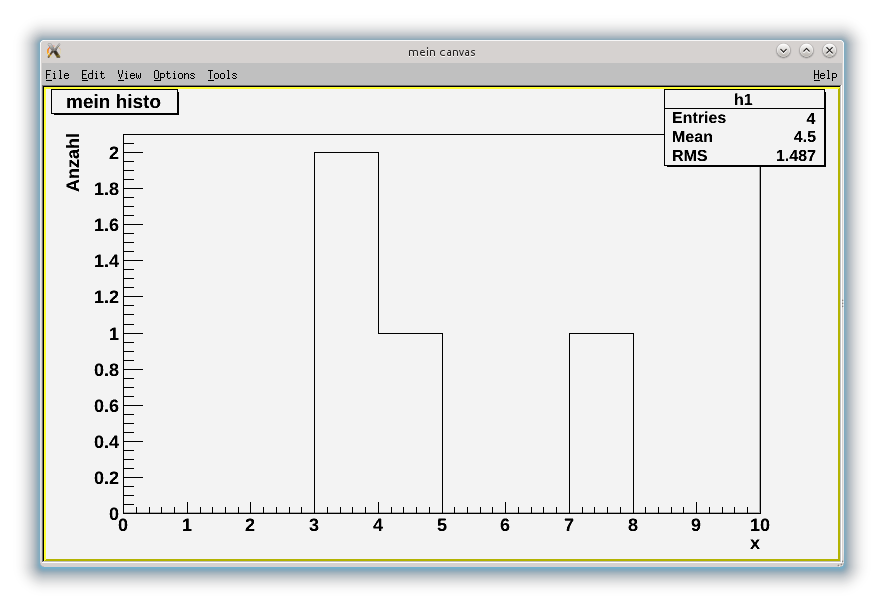
\includegraphics[width=10cm]{Uebung_10/default.png}
\caption{Standardplot}
\end{center}
\end{figure}



\begin{figure}[h]
\begin{center}
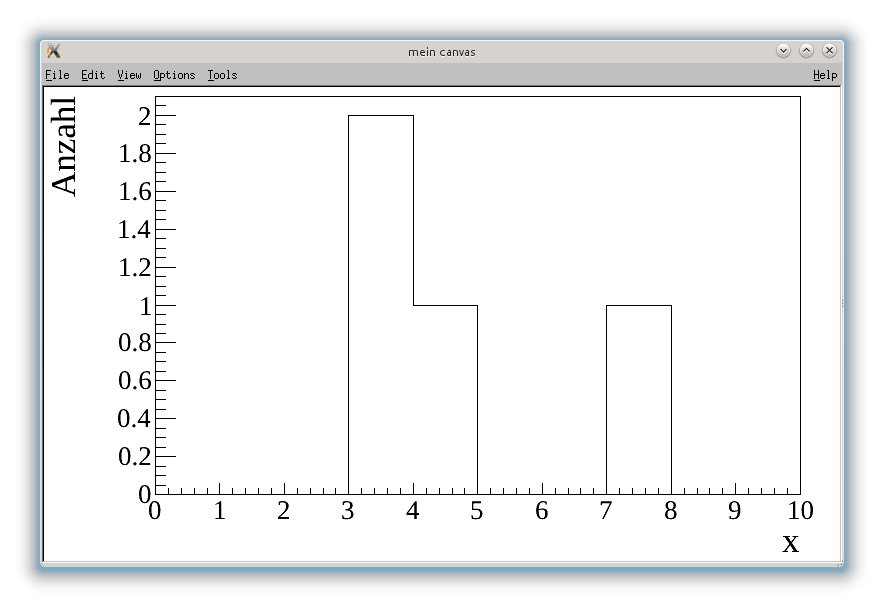
\includegraphics[width=10cm]{Uebung_10/babar.png}
\caption{BABAR Plot}
\end{center}
\end{figure}

Man kann mit \texttt{c1->SetLogx(1)} eine logarithmische Achse aktivieren und mit \texttt{c1->SetLogx(0)} wieder zurück zur linearen Achse wechseln.

\section{Berichtsaufgabe}

Man kann hier einfach den entsprechenden Konstruktor benutzen, da die Datei freundlichweise schon passend formatiert ist.

\code[c++]{Uebung_10/bericht.C}{Code fuer Plot}{code:root1}

ROOT gibt dann folgende Parameter für den Fit aus (Tablle \ref{table:fit}).

\begin{table}[h]
\begin{center}
\begin{tabular}{lcrcr}
Chi2 & = & $48.4851$ &  \\ 
NDf & = & $17$ &  \\ 
p0 & = & $-0.153455$ & $\pm$ & $0.0434887$ \\ 
p1 & = & $2.04459$ & $\pm$ & $0.00707916$ \\ 
\end{tabular} 
\caption{Parameter des Fits}
\label{table:fit}
\end{center}
\end{table}

ROOT zeichnet auch direkt die Linie ein. Man kann ihr Erscheinungsbild in der GUI dann auch noch verändern.


\begin{figure}[h]
\begin{center}
\includegraphics[width=14cm]{Uebung_10/histogram.pdf}
\caption{Messwerte mit linearem Fit}
\end{center}
\end{figure}

\section{Kugel im Öltank}

Für $\alpha \neq 0$ kann man die Funktionen einfach plotten. Für die kleine Masse habe ich blaue Farbe benutzt, für $m=\unit[1{,}5]{kg}$ rote Farbe. Das kleine $\alpha$ ist mit einer dünnen Linie, das große $\alpha$ mit einer dicken Linie dargestellt. Die ganz dünne schwarze Linie zeigt $\alpha = 0$.

Dabei braucht man gar nicht die Taylorreihe zu entwickeln, sondern auf den Aufgabenzettel der Physik zu schauen. Dort hat man bereits die Formel

\begin{equation*}
\dot{\vec{v}} = \vec{g} - \frac{\alpha}{m} \vec{v}
\end{equation*}

hergeleitet. Fällt das $\alpha$ weg, so hat man einfach nur eine ganz normale Fallbewegung. Dann braucht man nur noch $v(t) = g*t$ einzutragen.

\begin{figure}[h]
\begin{center}
\includegraphics[width=14cm]{Uebung_10/kugel.pdf}
\caption{Zeit-Geschwindigkeits Plot für die Kugel im Öltank}
\end{center}
\end{figure}

\code[c++]{Uebung_10/kugel.C}{Code für Kugelaufgabe}{code:root-kugel}
